\documentclass[11pt,twoside]{article}

\usepackage{amsmath,amsthm}
\usepackage[headings]{fullpage}
\usepackage[utopia]{mathdesign}
\usepackage{color}
\usepackage{graphicx}

\pagestyle{myheadings}
\markboth{Pressure fit}{Pressure fit}

\usepackage{amsmath}
\usepackage{bm}

\newcommand{\nat}{\mathbb{N}}          % Natural numbers
\newcommand{\integer}{\mathbb{Z}}      % Integers
\newcommand{\real}{ {\mathbb{R}} }     % Reals
\newcommand{\float}{ {\mathbb{F}} }     % Reals
\newcommand{\rmn}[2]{ \mathbb{R}^{#1\times#2} }     % Reals
\newcommand{\complex}{ {\mathbb{C}} }  % Complex
\newcommand{\macheps}{\ensuremath \varepsilon_{\text{mach}}}

\renewcommand{\Re}{\operatorname{Re}}
\renewcommand{\Im}{\operatorname{Im}}

% Boldface vectors
\newcommand{\bff}{\bm{f}}
\newcommand{\bfF}{\bm{F}}
\newcommand{\bfw}{\bm{w}}
\newcommand{\bfv}{\bm{v}}
\newcommand{\bfe}{\bm{e}}
\newcommand{\bfc}{\bm{c}}
\newcommand{\bfp}{\bm{p}}
\newcommand{\bfq}{\bm{q}}
\newcommand{\bfr}{\bm{r}}
\newcommand{\bfs}{\bm{s}}
\newcommand{\bfu}{\bm{u}}
\newcommand{\bfb}{\bm{b}}
\newcommand{\bfx}{\bm{x}}
\newcommand{\bfy}{\bm{y}}
\newcommand{\bfg}{\bm{g}}
\newcommand{\bfh}{\bm{h}}
\newcommand{\bfz}{\bm{z}}
\newcommand{\bfa}{\bm{a}}
\newcommand{\bft}{\bm{t}}
\newcommand{\bfd}{\bm{d}}
\newcommand{\bfalpha}{\bm{\alpha}}
\newcommand{\bfeps}{\bm{\varepsilon}}
\newcommand{\bfdelta}{\bm{\delta}}
\newcommand{\bfzero}{\bm{0}}
\newcommand{\eye}[1]{\bfe_{#1}}

% Boldface matrix
\newcommand{\m}[1]{\bm{#1}}
\newcommand{\mA}{\m{A}}
\newcommand{\mL}{\m{L}}
\newcommand{\mF}{\m{F}}
\newcommand{\mU}{\m{U}}
\newcommand{\mJ}{\m{J}}
\newcommand{\mP}{\m{P}}
\newcommand{\mQ}{\m{Q}}
\newcommand{\mR}{\m{R}}
\newcommand{\mD}{\m{D}}
\newcommand{\mS}{\m{S}}
\newcommand{\mB}{\m{B}}
\newcommand{\mC}{\m{C}}
\newcommand{\mE}{\m{E}}
\newcommand{\mG}{\m{G}}
\newcommand{\mH}{\m{H}}
\newcommand{\mV}{\m{V}}
\newcommand{\mW}{\m{W}}
\newcommand{\mX}{\m{X}}
\newcommand{\mZ}{\m{Z}}
\newcommand{\mK}{\m{K}}
\newcommand{\mM}{\m{M}}

\newcommand{\meye}{\m{I}}

\newcommand{\ee}[1]{\times 10^{#1}}
\newcommand{\jac}[2]{\frac{\bfd \bm{#1}}{\bfd \bm{#2}}}
\newcommand{\diag}{\operatorname{diag}}
\newcommand{\fl}{\operatorname{fl}}
\newcommand{\circop}[1]{\makebox[0pt][l]{$\bigcirc$}\hspace{1pt}#1}
\newcommand{\myvec}{\operatorname{vec}}
\newcommand{\unvec}{\operatorname{unvec}}
\newcommand{\kron}[2]{#1 \otimes #2}


\begin{document}

\begin{center}
  \bf Grace under pressure
\end{center}

This figure represents arterial blood pressure collected at 8 ms intervals
from an infant patient:
\begin{center}
  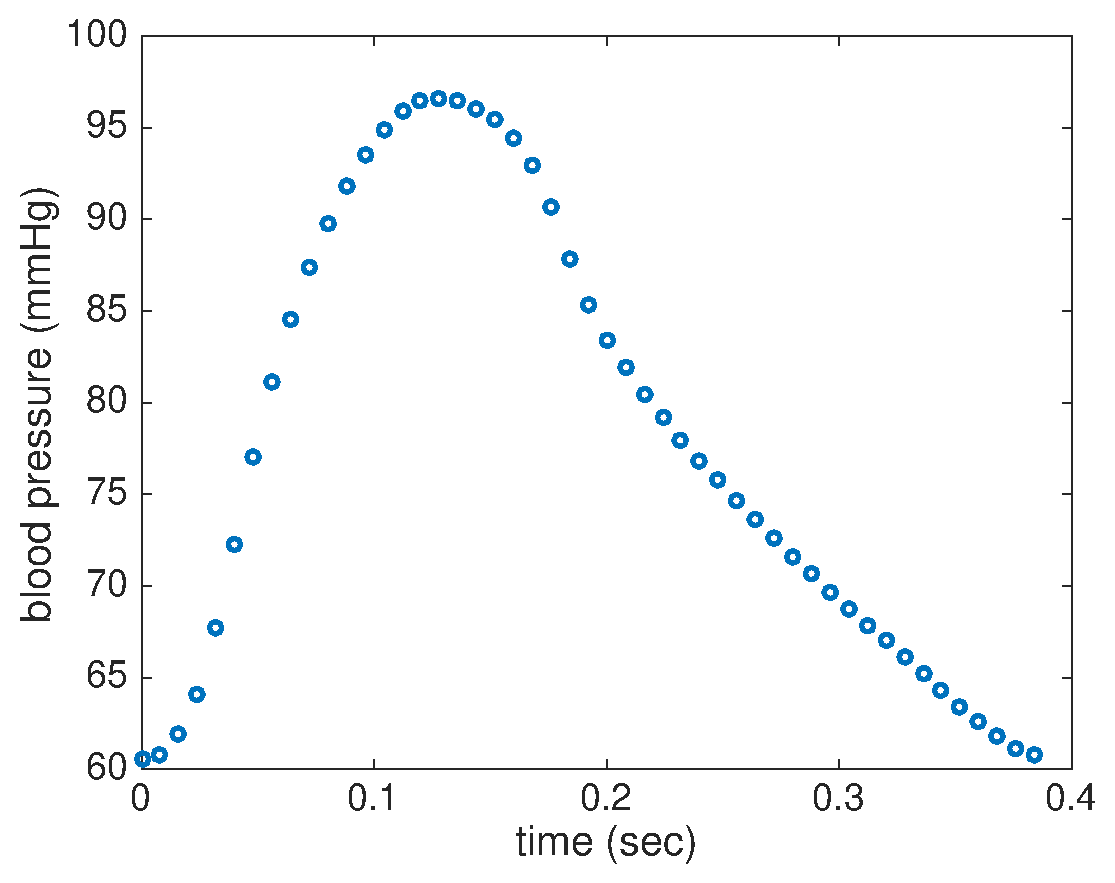
\includegraphics[height=2.5in]{fitfigure}
\end{center}
Call these points $(t_i,y_i)$ for $i=1,\ldots,m$. The numerical data
can be found on the website.

These data can be fit using a function of the form
\begin{equation}
  \label{eq:1}
  f(t) = c_1 f_1(t) + c_2 f_2(t) + \cdots + c_nf_n(t),
\end{equation}
for functions $f_1,\ldots,f_n$ that are predetermined and coefficients $c_1,\ldots,c_n$ that are chosen to optimize the fit to the data. This optimization can be formulated as an $m\times n$ linear least-squares problem of minimizing $\|\bfy-\mA\bfc\|_2$, where $A_{ij} = f_j(t_i)$.

Typical choices for the functions $f_j$ are monomials, $f_j(t)=t^{j-1}$ for $j=1,\ldots,n$. These lead to polynomial fits, the classic case being a straight line. Since here the data are taken over one heartbeat, they are roughly periodic in time. That fact can be exploited to produce a fit. Let $T = t_m-t_1$ be the period of the beat. Then one periodic fit is
\begin{equation}
  \label{eq:2}
  f(t) = c_1 + c_2 \cos\left(\frac{2\pi t}{T}\right) +  c_3 \sin\left(\frac{2\pi t}{T}\right) + c_4 \cos\left(\frac{4\pi t}{T}\right) +  c_5 \sin\left(\frac{4\pi t}{T}\right).
\end{equation}

\subsection*{Goals}

You will fit the real-world data in the graph above using different least squares approximations.

\subsection*{Preparation}

Read section 3.1. 

\subsection*{Procedure}

Download the template and the file \texttt{pressuredata.mat}. Fill out the template so that it performs the following steps. 

\begin{enumerate}
\item Load the data into MATLAB using \texttt{load pressuredata}. This creates two vectors \texttt{t} and \texttt{y} containing the data. Use them to recreate the plot above.

\item The most popular type of fit is to a straight line, for which  $n=2$ and $f_1(t)=1$, $f_2(t)=t$. Even though this data will clearly not be well represented as a straight line, go through the motions anyway and solve for the optimal coefficients using backslash. Superimpose the graph of the line on your graph from the previous step, and compute the residual norm $\|\bfy-\mA\bfc\|_2$ at the solution $\bfc$.

\item Repeat step 2 for a quadratic polynomial and a cubic polynomial. The residual norm will get smaller in each case, but you will see that these fits still leave much to be desired.

\item Create the fit suggested by~\eqref{eq:2} and add it to the plot. Based on the residual norm, is this better than the polynomial fits? 
  
\end{enumerate}


\end{document}

%%% Local Variables: 
%%% mode: latex
%%% TeX-master: t
%%% End: 
